\documentclass[a4paper,11pt]{article}
\usepackage[dvipsnames,table]{xcolor}
\usepackage[a4paper,margin=2.5cm,headheight=15pt]{geometry}
\usepackage[utf8]{inputenc}
\usepackage[T1]{fontenc}
\usepackage[serbian]{babel}
\usepackage{lmodern,microtype}
\usepackage{amsmath,amssymb,mathtools}
\numberwithin{equation}{section}
\usepackage{graphicx,adjustbox,placeins}
\graphicspath{{Images/}}
\usepackage{booktabs,tabularx,longtable,array,multirow,makecell}
\usepackage{caption,subcaption}
\captionsetup{font=small,labelfont=bf}
\usepackage{siunitx}
\sisetup{detect-all}
\usepackage[most]{tcolorbox}
\usepackage{enumitem}
\setlist{nosep}
\usepackage{fancyhdr}
\definecolor{Primary}{HTML}{1F77B4}
\definecolor{Accent}{HTML}{2CA02C}
\usepackage[colorlinks=true,linkcolor=Primary,citecolor=Primary,urlcolor=Primary]{hyperref}
\usepackage{cleveref}
\pagestyle{fancy}
\fancyhf{}
\lhead{\small\textit{Statičke karakteristike logičkih kola}}
\rhead{\thepage}
\renewcommand{\arraystretch}{1.25}
\newcolumntype{C}{>{\centering\arraybackslash}X}
\renewcommand{\contentsname}{Sadržaj}
\setlength{\emergencystretch}{2em}
\allowdisplaybreaks[2]
\newcommand{\napomena}[1]{\begin{tcolorbox}[colback=gray!10,colframe=black,boxrule=0.5pt]#1\end{tcolorbox}}
\newcommand{\redlinija}{\arrayrulecolor{black!28}\specialrule{0.3pt}{2pt}{2pt}\arrayrulecolor{black}}
\newcommand{\kod}[1]{\ensuremath{\mathtt{#1}}}
\begin{document}
\hypersetup{pageanchor=false}
\begin{titlepage}
\thispagestyle{empty}
\begin{center}
{\Large\bfseries UNIVERZITET U BEOGRADU -- ELEKTROTEHNIČKI FAKULTET\\ KATEDRA ZA ELEKTRONIKU\par}
\vspace{25mm}
{\LARGE\bfseries DIGITALNA ELEKTRONIKA 1\par}
\vspace{2mm}
{\large Materijali za računske vežbe\par}
\vspace{18mm}
{\Large\bfseries STATIČKE KARAKTERISTIKE LOGIČKIH KOLA\par}
\vspace{3mm}
{\large Vežbe 7\par}
\vfill
\begin{minipage}{0.62\linewidth}
\raggedright\textbf{Autori:}\\[4pt]\small
\begin{tabular}{@{}ll@{}}
Nikola Petrović & \href{mailto:p.z.nikola@etf.bg.ac.rs}{\texttt{p.z.nikola@etf.bg.ac.rs}}\\
Haris Turkmanović & \href{mailto:haris@etf.bg.ac.rs}{\texttt{haris@etf.bg.ac.rs}}\\
\end{tabular}
\end{minipage}\hfill
\begin{minipage}{0.34\linewidth}\raggedleft Beograd, \today\end{minipage}
\end{center}
\end{titlepage}
\hypersetup{pageanchor=true}
\tableofcontents
\newpage
\section{Zadatak 1: kaskada invertora}\label{sec:1}
Karakteristika prenosa invertora napajanog naponom $V_{CC}=5\,\mathrm V$ prikazana je na slici~\ref{fig:1.1}. Za kaskadu proizvoljno velikog parnog broja istih kola i ulaz $v_0=1.75\,\mathrm V$ grafički odrediti granični izlazni napon.
\begin{figure}[!htbp]\centering
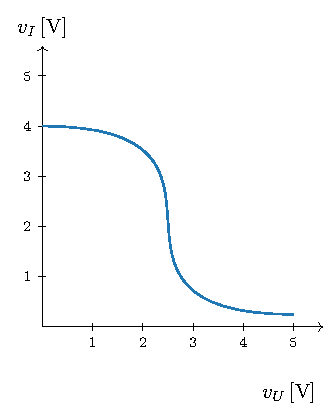
\includegraphics[width=.48\linewidth]{Zadatak_1/karakteristika}
\caption{Zadata karakteristika invertora; skala je u voltima.}\label{fig:1.1}
\end{figure}
\subsection*{Rešenje}
Ako je $f$ karakteristika jednog kola, izlaz stepena $k$ istovremeno je ulaz narednog stepena:
\begin{equation}\label{eq:1.1}
v_k=f(v_{k-1}),\qquad v_0=1.75\,\mathrm V.
\end{equation}

Prvo očitamo $v_1=f(v_0)$, zatim $v_2=f(v_1)$, pa $v_3$ i $v_4$. Konstrukcija je data na slici~\ref{fig:1.2}. Isti postupak može se prikazati sa četiri kopije karakteristike, sukcesivno zarotirane za $90^\circ$: izlazna osa jednog kola postaje ulazna osa sledećeg (slika~\ref{fig:1.3}).
\begin{figure}[!htbp]\centering
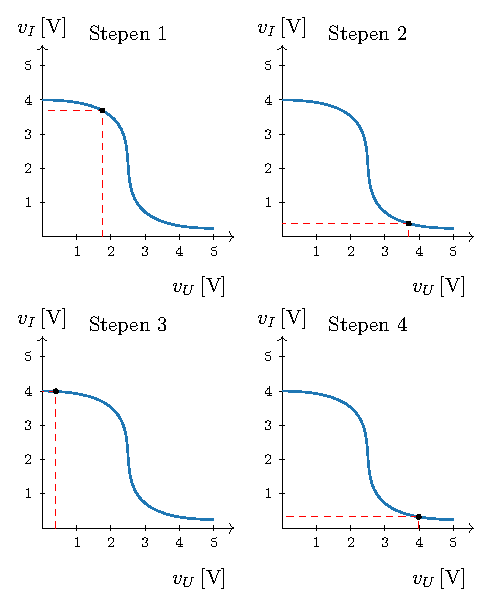
\includegraphics[width=.8\linewidth]{Zadatak_1/iteracije}
\caption{Prva četiri koraka grafičkog određivanja napona.}\label{fig:1.2}
\end{figure}\begin{figure}[!htbp]\centering
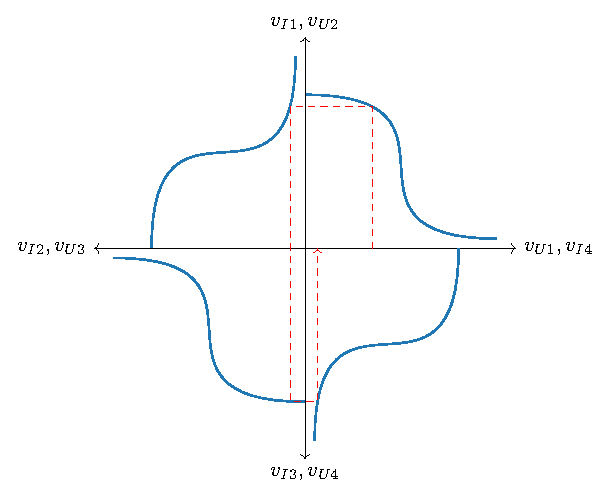
\includegraphics[width=.7\linewidth]{Zadatak_1/rotacija}
\caption{Grafička iteracija sa četiri zarotirane karakteristike.}\label{fig:1.3}
\end{figure}
Još pregledniji prikaz dobija se preslikavanjem karakteristike u odnosu na pravu $v_I=v_U$ (slika~\ref{fig:1.4}). Preseci van dijagonale određuju par stabilnih nivoa $(V_L,V_H)$ i $(V_H,V_L)$, za koje važi $f(V_L)=V_H$, $f(V_H)=V_L$. Presek na dijagonali određuje prag $V_S=f(V_S)$; za prikazanu karakteristiku on je nestabilan. Oblasti između krive i njenog odraza usmeravaju iteraciju ka stabilnim nivoima, što predstavlja regeneraciju.
Pošto je zadati ulaz ispod praga, neparni izlazi teže visokom, a parni niskom nivou:
\begin{equation}\label{eq:1.2}
\lim_{n\to\infty}v_{2n}=V_L,\qquad \lim_{n\to\infty}v_{2n+1}=V_H.
\end{equation}

\napomena{Izvor daje samo crtež, bez analitičke funkcije ili dovoljno numeričkih tačaka. Zato je odgovor grafički: niski nivo iznosi nekoliko desetih delova volta. Ne treba ga poistovećivati sa tačno $0\,\mathrm V$, niti visoki nivo sa napajanjem $5\,\mathrm V$. Ponovo nacrtana kriva čuva oblik izvornika; iz nje se ne izvodi prividno precizan numerički rezultat.}
\begin{figure}[!htbp]\centering
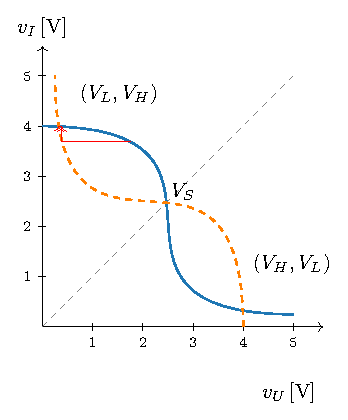
\includegraphics[width=.65\linewidth]{Zadatak_1/preslikavanje}
\caption{Karakteristika, njen odraz i približavanje stabilnom paru nivoa.}\label{fig:1.4}
\end{figure}
\FloatBarrier\section{Zadatak 2: margine šuma}\label{sec:2}
Za invertor u lancu istih kola odrediti margine šuma za: a) jedan izvor šuma; b) izvore šuma na svim međuspojevima. Karakteristični nivoi prikazani su na slici~\ref{fig:2.1}.
\subsection*{Rešenje}
Koristimo oznake $V_L,V_H$ za stabilne nivoe u lancu bez šuma. Oznake $V_{OL},V_{OH}$ rezervisane su za garantovane granice izlaza pri dozvoljenim ulazima. U izvorniku su obe vrste nivoa označene istim simbolima; razlika je važna kada krajnji segmenti nisu horizontalni.
\begin{figure}[!htbp]\centering
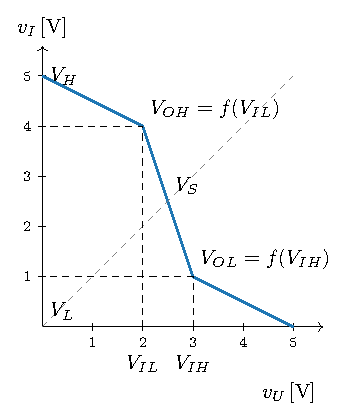
\includegraphics[width=.7\linewidth]{Zadatak_2/nivoi}
\caption{Ulazni pragovi, garantovani izlazni nivoi i stabilni nivoi (ilustrativna karakteristika).}\label{fig:2.1}
\end{figure}
\paragraph{a) Jednostruki izvor šuma (SSNM).}
Šum amplitude $V_N$ deluje na ulazu samo jednog invertora. Ako je prethodni izlaz visok, najnepovoljniji šum ga umanjuje; ako je nizak, uvećava ga. Za očuvanje logičke informacije potrebno je ostati sa odgovarajuće strane praga:
\begin{equation}\label{eq:2.1}
V_H-V_N>V_S,
\end{equation}
\begin{equation}\label{eq:2.2}
V_L+V_N<V_S.
\end{equation}
\begin{figure}[!htbp]\centering
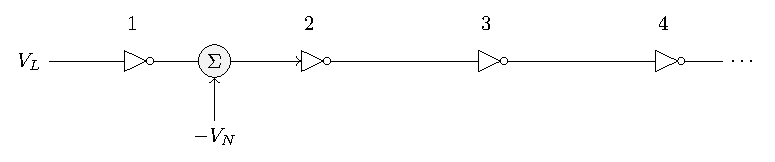
\includegraphics[width=0.9\linewidth]{Zadatak_2/jednostruki}
\caption{Šum na jednoj međuvezi u lancu invertora.}\label{fig:2.2}
\end{figure}
Naredni stepeni regenerišu poremećeni nivo. Granične amplitude su
\begin{equation}\label{eq:2.6}
NM_{0,\mathrm{SS}}=V_S-V_L,\qquad NM_{1,\mathrm{SS}}=V_H-V_S.
\end{equation}

Jednakost sa pragom ne garantuje odluku; u idealnom modelu može zadržati radnu tačku na nestabilnom preseku.
\paragraph{b) Višestruki izvori šuma (MSNM).}
Kada šum postoji na svakoj međuvezi, prihvatljivi ulazi moraju ostati u oblastima malog pojačanja. Lokalni uslov slabljenja perturbacije je
\begin{equation}\label{eq:2.3}
\left|\frac{\mathrm d f}{\mathrm d v_U}\right|<1.
\end{equation}

Za glatku karakteristiku granice $V_{IL},V_{IH}$ određene su nagibom $-1$. Kod izlomljene karakteristike uzimaju se prelomi na kojima modul nagiba prelazi jedinicu. Uslovi očuvanja dozvoljenih intervala su
\begin{equation}\label{eq:2.4}
f(V_{IH})+V_N<V_{IL},
\end{equation}
\begin{equation}\label{eq:2.5}
f(V_{IL})-V_N>V_{IH}.
\end{equation}
\begin{figure}[!htbp]\centering
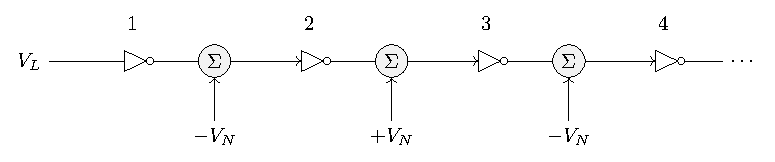
\includegraphics[width=0.9\linewidth]{Zadatak_2/visestruki}
\caption{Najnepovoljniji znaci šuma na uzastopnim međuspojevima.}\label{fig:2.3}
\end{figure}
Za monotonu opadajuću karakteristiku garantovani nivoi i pripadne margine glase
\begin{equation}\label{eq:2.7}
\begin{gathered}V_{OL}=f(V_{IH}),\qquad V_{OH}=f(V_{IL}),\\ NM_0=V_{IL}-V_{OL},\qquad NM_1=V_{OH}-V_{IH}.\end{gathered}
\end{equation}

Ako su krajnji delovi skoro horizontalni, dozvoljena je dodatna aproksimacija $f(V_{IH})\approx V_L$, $f(V_{IL})\approx V_H$, pa
\begin{equation}\label{eq:2.8}
NM_0\approx V_{IL}-V_L,\qquad NM_1\approx V_H-V_{IH}.
\end{equation}

Ovo nisu opšte tačne jednakosti. SSNM je koristan za razumevanje regeneracije i projektovanje samog kola; garantovane margine pri poremećajima na svim međuspojevima koriste se pri povezivanju kola. U svim sledećim zadacima prikazane su i tačne vrednosti prema~\eqref{eq:2.7} i procene prema~\eqref{eq:2.8} iz izvornika.
\FloatBarrier\section{Zadatak 3: tri invertorske karakteristike}\label{sec:3}
Tri tipa kola sa slike~\ref{fig:3.1} napajaju se sa $5\,\mathrm V$. U svakom lancu nalaze se ista kola. Za ulaz $2.7\,\mathrm V$: a) odrediti izlaze posle beskonačno mnogo parova kola; b) oceniti pogodnost za logičko NE kolo; c) za pogodno kolo odrediti nivoe, prag i obe vrste margina šuma.
\begin{figure}[!htbp]\centering
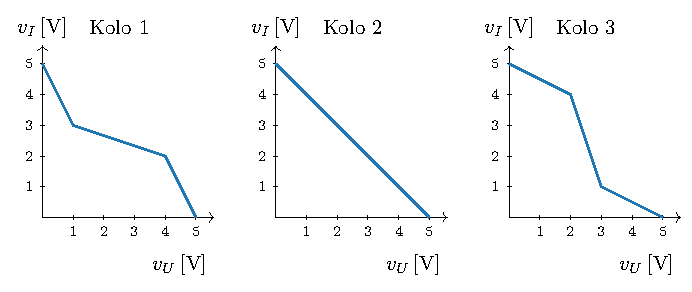
\includegraphics[width=\linewidth]{Zadatak_3/karakteristike}
\caption{Tri invertorske karakteristike.}\label{fig:3.1}
\end{figure}
\subsection*{Rešenje}
U formulama koje slede, $x=v_U/(1\,\mathrm V)$, a funkcije daju brojnu vrednost izlaza u voltima:
\begin{equation}\label{eq:3.1}
\begin{aligned} f_1(x)&=\begin{cases}5-2x,&0\le x\le1,\\(10-x)/3,&1\le x\le4,\\2(5-x),&4\le x\le5;\end{cases}\\ f_2(x)&=5-x;\\ f_3(x)&=\begin{cases}5-x/2,&0\le x\le2,\\10-3x,&2\le x\le3,\\(5-x)/2,&3\le x\le5.\end{cases}\end{aligned}
\end{equation}

\paragraph{a) Izlazi lanaca.}
Za prvo kolo početna tačka i sve naredne tačke ostaju na srednjem segmentu. Iz $v_k-2.5\,\mathrm V=-(v_{k-1}-2.5\,\mathrm V)/3$ sledi
\begin{equation}\label{eq:3.2}
v_k-2.5\,\mathrm V=\left(-\frac13\right)^k(v_0-2.5\,\mathrm V),\qquad \lim_{n\to\infty}v_{2n}=2.5\,\mathrm V.
\end{equation}

Za drugo kolo $v_{2n}=2.7\,\mathrm V$, a $v_{2n+1}=2.3\,\mathrm V$. Parni podniz ima granicu $2.7\,\mathrm V$, dok ceo niz nema granicu. Za treće kolo parni izlazi teže $5\,\mathrm V$, a neparni $0\,\mathrm V$.
\paragraph{b) Regeneracija.}
Prvo kolo smanjuje odstupanje od sredine tri puta po stepenu. Ako je ulaz na krajnjem segmentu, odstupanje od odgovarajuće šine raste: za mali pozitivan $v_0$, dok se prolazi kroz krajnje segmente, $v_2=4v_0$, $v_4=16v_0$. Tačka zato dospeva na srednji segment i teži $2.5\,\mathrm V$. Izuzetak je idealni par $0\leftrightarrow5\,\mathrm V$, koji je nestabilan. Takvo kolo gubi informaciju o logičkom nivou.
Drugo kolo ima modul nagiba jedan i ne umanjuje odstupanja. Ni ono ne obezbeđuje regeneraciju.
Treće kolo na krajnjim segmentima ima modul nagiba $1/2$, pa smanjuje odstupanja od šina. Srednji segment ima nagib $-3$, pa odbija tačku od $2.5\,\mathrm V$ prema jednoj od dve stabilne oblasti. Tačno $2.5\,\mathrm V$ ostaje nestabilna fiksna tačka. Samo treće kolo je pogodno za NE funkciju.
\paragraph{c) Nivoi i margine trećeg kola.}
\begin{figure}[!htbp]\centering

\includegraphics[width=.6\linewidth]{Zadatak_3/preslikavanje}
\caption{Treća karakteristika i njen odraz u odnosu na dijagonalu.}\label{fig:3.2}
\end{figure}\begin{equation}\label{eq:3.3}
V_L=0,\quad V_H=5\,\mathrm V,\quad V_S=2.5\,\mathrm V,\quad V_{IL}=2\,\mathrm V,\quad V_{IH}=3\,\mathrm V.
\end{equation}
\begin{equation}\label{eq:3.4}
NM_{0,\mathrm{SS}}=NM_{1,\mathrm{SS}}=2.5\,\mathrm V.
\end{equation}
\begin{equation}\label{eq:3.5}
V_{OL}=f_3(3)\,\mathrm V=1\,\mathrm V,\quad V_{OH}=f_3(2)\,\mathrm V=4\,\mathrm V,\quad NM_0=NM_1=1\,\mathrm V.
\end{equation}

Procena koja zamenjuje garantovane izlaze šinama daje $2\,\mathrm V$ za obe margine. Ovde krajnji nagib iznosi $1/2$, pa ta procena precenjuje garantovane margine za $1\,\mathrm V$.
\FloatBarrier\section{Zadatak 4: tri baferske karakteristike}\label{sec:4}
Za tri baferska kola sa slike~\ref{fig:4.1}, napajana sa $5\,\mathrm V$, ponoviti analizu prethodnog zadatka za ulaz $2.7\,\mathrm V$ i beskonačan lanac istih kola: a) izlaz; b) regeneracija; c) nivoi, prag i margine.
\begin{figure}[!htbp]\centering

\includegraphics[width=\linewidth]{Zadatak_4/karakteristike}
\caption{Tri baferske karakteristike.}\label{fig:4.1}
\end{figure}
\subsection*{Rešenje}
\paragraph{Opšti postupak za linearan segment.}
Segment je oblika $y=kx+C$. Ako svi stepeni ostaju na istom segmentu, za $k\ne1$:
\begin{equation}\label{eq:4.1}
y_n=k^n x_0+C\sum_{j=0}^{n-1}k^j=k^n x_0+C\frac{k^n-1}{k-1}=y_*+k^n(x_0-y_*),\qquad y_*=\frac{C}{1-k}.
\end{equation}
\begin{figure}[!htbp]\centering
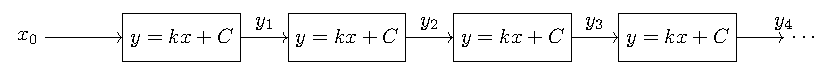
\includegraphics[width=0.9\linewidth]{Zadatak_4/lanac}
\caption{Iteracija istog linearnog segmenta.}\label{fig:4.2}
\end{figure}
Za $|k|<1$ izlaz teži $y_*$, preseku segmenta sa $y=x$. Za $k>1$ odstupanje od $y_*$ raste ako $x_0\ne y_*$; smer rasta zavisi od znaka tog odstupanja. Matematička prava bi dala neograničen izlaz, ali u stvarnom kolu tačka prelazi na drugi segment i napon ostaje ograničen napajanjem. Za $k=1,C=0$ važi $y_n=x_0$. Za $k=1,C\ne0$ važi $y_n=x_0+nC$, dok se ne napusti segment. Za $k=-1$ nastaje dvociklus, osim u fiksnoj tački; za $k<-1$ odstupanja rastu uz promenu znaka. Uslov za konvergenciju nije samo $k<1$.
\paragraph{a) Izlazi.}
Uz istu normalizaciju kao ranije,
\begin{equation}\label{eq:4.2}
\begin{aligned} b_1(x)&=\begin{cases}2x,&0\le x\le1,\\(x+5)/3,&1\le x\le4,\\2x-5,&4\le x\le5;\end{cases}\\b_2(x)&=x;\\ b_3(x)&=\begin{cases}x/2,&0\le x\le2,\\3x-5,&2\le x\le3,\\(x+5)/2,&3\le x\le5.\end{cases}\end{aligned}
\end{equation}

Prvi lanac teži $2.5\,\mathrm V$, drugi ostaje na $2.7\,\mathrm V$, a treći teži $5\,\mathrm V$.
\paragraph{b) Regeneracija.}
Prvo kolo privlači tačke sredini, a drugo zadržava svaku ulaznu vrednost. Treće kolo obnavlja niski ili visoki nivo, jer je nagib $1/2$ u krajnjim oblastima, a $3$ oko praga. Samo ono je pogodno kao logički bafer.
\paragraph{c) Nivoi i margine.}
Stabilni nivoi su $V_L=0$, $V_H=5\,\mathrm V$, prag $V_S=2.5\,\mathrm V$, a granice $V_{IL}=2\,\mathrm V$, $V_{IH}=3\,\mathrm V$. Obe SSNM margine iznose $2.5\,\mathrm V$. Za rastuću karakteristiku garantovane izlaze računamo na istoimenim ulaznim granicama:
\begin{equation}\label{eq:4.3}
V_{OL}=b_3(2)\,\mathrm V=1\,\mathrm V,\quad V_{OH}=b_3(3)\,\mathrm V=4\,\mathrm V,\quad NM_0=NM_1=1\,\mathrm V.
\end{equation}

Izvorna procena zasnovana na stabilnim nivoima daje $2\,\mathrm V$; ovde nije tačna garantovana margina.
\FloatBarrier\section{Zadatak 5: karakteristika kaskade}\label{sec:5}
Odrediti karakteristiku kaskade dva kola sa slike~\ref{fig:5.1}, redom invertora pa bafera, kao i nivoe, prag i margine za jednostruki i višestruke izvore šuma.
\begin{figure}[!htbp]\centering

\includegraphics[width=0.9\linewidth]{Zadatak_5/karakteristike}
\caption{Invertor i bafer koji se povezuju redno.}\label{fig:5.1}
\end{figure}
\subsection*{Rešenje}
Prvo kolo ima karakteristiku $f_3$, a drugo $b_3$ iz~\eqref{eq:3.1} i~\eqref{eq:4.2}. Njihovi segmenti su redom $5-x/2$, $10-3x$, $(5-x)/2$, odnosno $x/2$, $3x-5$, $(x+5)/2$. Rotacijom druge karakteristike za $90^\circ$ dobija se grafička konstrukcija sa slike~\ref{fig:5.2}.
\begin{figure}[!htbp]\centering

\includegraphics[width=0.9\linewidth]{Zadatak_5/rotacija}
\caption{Preslikavanje karakterističnih tačaka kroz oba kola.}\label{fig:5.2}
\end{figure}
Pošto su obe karakteristike deo po deo linearne, dovoljno je odrediti sve prelomne tačke kompozicije $h=b_3\circ f_3$ i spojiti susedne tačke:
\begin{center}\begin{tabular}{cccc}\toprule
Tačka & $v_U\,[\mathrm V]$ & $v_{I1}\,[\mathrm V]$ & $v_I\,[\mathrm V]$\\
\midrule
Početak & 0 & 5 & 5\\
\redlinija
$T_1$ & 2 & 4 & $9/2$\\
\redlinija
$T_2$ & $7/3$ & 3 & 4\\
\redlinija
$T_3$ & $8/3$ & 2 & 1\\
\redlinija
$T_4$ & 3 & 1 & $1/2$\\
\redlinija
Kraj & 5 & 0 & 0\\
\bottomrule\end{tabular}\end{center}
Za $T_1$ ulaz $2\,\mathrm V$ daje međunapon $4\,\mathrm V$, pa izlaz $4.5\,\mathrm V$. Za $T_2$ međunapon mora biti $3\,\mathrm V$, otuda $10-3x=3$ i $x=7/3$. Analogno se dobijaju $T_3$ i $T_4$. Dobijena karakteristika je
\begin{equation}\label{eq:5.1}
h(x)=\begin{cases}5-x/4,&0\le x\le2,\\15/2-3x/2,&2\le x\le7/3,\\25-9x,&7/3\le x\le8/3,\\5-3x/2,&8/3\le x\le3,\\5/4-x/4,&3\le x\le5.\end{cases}
\end{equation}
\begin{figure}[!htbp]\centering
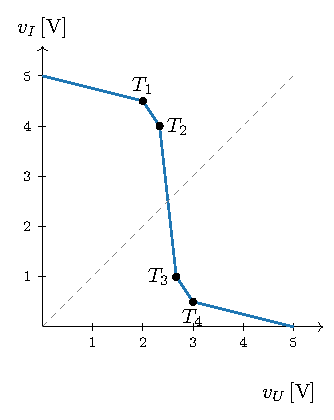
\includegraphics[width=.65\linewidth]{Zadatak_5/rezultat}
\caption{Prenosna karakteristika kaskade sa četiri unutrašnja preloma.}\label{fig:5.3}
\end{figure}
Moduli nagiba su $1/4,3/2,9,3/2,1/4$. Granice dozvoljenih ulaza zato su $V_{IL}=2\,\mathrm V$ i $V_{IH}=3\,\mathrm V$. Stabilni nivoi su $V_L=0$ i $V_H=5\,\mathrm V$, a prag $V_S=2.5\,\mathrm V$. Obe SSNM margine iznose $2.5\,\mathrm V$. Garantovani izlazi i margine su
\begin{equation}\label{eq:5.2}
V_{OL}=h(3)\,\mathrm V=0.5\,\mathrm V,\quad V_{OH}=h(2)\,\mathrm V=4.5\,\mathrm V,\quad NM_0=NM_1=1.5\,\mathrm V.
\end{equation}

Procena sa stabilnim nivoima ponovo daje $2\,\mathrm V$. U ovom primeru ona precenjuje obe garantovane margine za $0.5\,\mathrm V$.

\end{document}
